\documentclass[11pt,a4paper]{article}

\usepackage[utf8]{inputenc}
\usepackage[T1]{fontenc}
\usepackage[ngerman]{babel}
\usepackage{lmodern}
\usepackage{amsmath,amssymb}
\usepackage{graphicx}
\usepackage{booktabs,tabularx,array}
\usepackage[table]{xcolor}
\usepackage{tikz}
\usetikzlibrary{arrows.meta,positioning,shapes.geometric,calc}
\usepackage[most]{tcolorbox}
\usepackage{enumitem}
\usepackage{microtype}
\usepackage{hyperref}
\usepackage[a4paper,left=18mm,right=18mm,top=15mm,bottom=15mm,headheight=0pt]{geometry}

\definecolor{navy}{HTML}{174A63}
\definecolor{blue}{HTML}{2E7698}
\definecolor{lightblue}{HTML}{EAF3F7}
\definecolor{lightgray}{HTML}{F2F3F4}
\definecolor{midgray}{HTML}{66727A}
\definecolor{green}{HTML}{477A63}
\definecolor{orange}{HTML}{B96A2B}

\hypersetup{colorlinks=true,linkcolor=navy,urlcolor=blue,pdftitle={Sicherungsblatt Aufgabe 1 -- Entscheidungsbäume}}
\setlength{\parindent}{0pt}
\setlength{\parskip}{4pt}
\setlist[itemize]{leftmargin=5mm,itemsep=1.5pt,topsep=2pt}
\setlist[enumerate]{leftmargin=6mm,itemsep=2pt,topsep=2pt}
\renewcommand{\familydefault}{\sfdefault}

\pagestyle{empty}

\newtcolorbox{definition}[1][]{enhanced,breakable,colback=lightblue,colframe=blue,
  boxrule=0.8pt,arc=1.5mm,left=3mm,right=3mm,top=2mm,bottom=2mm,
  fonttitle=\bfseries,title=Definition,#1}
\newtcolorbox{merke}[1][]{enhanced,breakable,colback=lightgray,colframe=navy,
  boxrule=0.9pt,arc=1.5mm,left=3mm,right=3mm,top=2mm,bottom=2mm,
  fonttitle=\bfseries,title=Merke,#1}
\newtcolorbox{beispiel}[1][]{enhanced,breakable,colback=white,colframe=midgray,
  boxrule=0.7pt,arc=1.5mm,left=3mm,right=3mm,top=2mm,bottom=2mm,
  fonttitle=\bfseries,title=Beispiel,#1}
\newtcolorbox{ueberblick}[1][]{enhanced,breakable,colback=lightblue,colframe=navy,
  boxrule=1.1pt,arc=1.5mm,left=3mm,right=3mm,top=2.5mm,bottom=2.5mm,
  fonttitle=\bfseries,title=Überblick,#1}

\newcommand{\fach}[1]{\textbf{\color{navy}#1}}
\newcommand{\sectionline}[1]{%
  \vspace{1mm}{\Large\bfseries\color{navy}#1}\par\vspace{1mm}%
  {\color{blue}\rule{\linewidth}{0.8pt}}\vspace{1mm}}
\newcommand{\sheettitle}[2]{%
  \begin{tcolorbox}[colback=navy,colframe=navy,arc=2mm,boxrule=0pt,left=5mm,right=5mm,top=2.5mm,bottom=2.5mm]
    {\color{white}\fontsize{20}{24}\selectfont\bfseries #1}\par
    \vspace{0.5mm}{\color{white}\large #2}
  \end{tcolorbox}}
\newcommand{\subline}[1]{\vspace{1mm}{\large\bfseries\color{navy}#1}\par}

\begin{document}

\sheettitle{Gutes Äffchen / Böses Äffchen}{Entscheidungsbäume · Sicherungsblatt zu Aufgabe 1 · Informatik 11}

\sectionline{1. Entscheidungsbäume}

Ein \fach{Entscheidungsbaum} ist ein Modell zur \fach{Klassifikation}: Er ordnet neue Daten anhand ihrer
Merkmale einer Klasse zu. Entscheidungsbäume können durch \fach{überwachtes Lernen} aus Beispielen mit
bekanntem Ergebnis erzeugt werden. Sie werden immer von oben nach unten durchlaufen.

\begin{definition}[title=Definition: Überwachtes Lernen]
Beim \fach{überwachten Lernen} wird aus \fach{gelabelten Daten} ein Modell erzeugt. Gelabelte Daten besitzen
neben ihren Merkmalen ein bekanntes \fach{Label}, also die richtige Klasse. Das Lernverfahren sucht Regeln,
mit denen es anschließend neue Eingaben klassifizieren kann.
\end{definition}

\begin{center}
  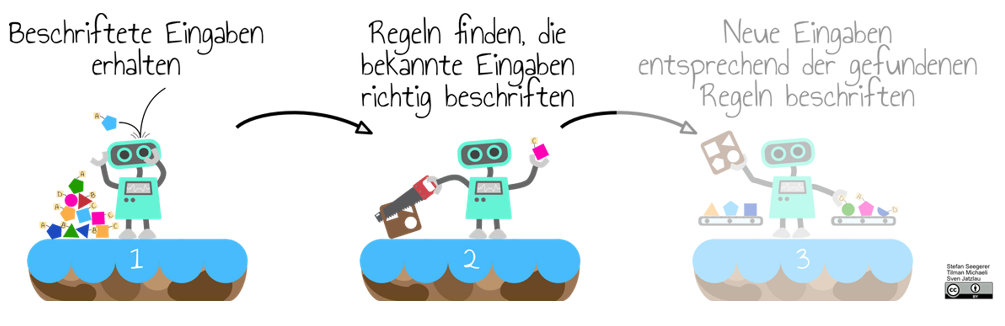
\includegraphics[width=0.76\linewidth]{sicherungsblatt-bilder/ueberwachtes-lernen.png}

  {\scriptsize\color{midgray}Abbildung: Stefan Seegerer, Tilman Michaeli und Sven Jatzlau, CC BY; übernommen aus dem Ausgangsmaterial.}
\end{center}

\sectionline{2. Aufbau eines Entscheidungsbaums}

\begingroup\small
\begin{center}
\begin{tikzpicture}[scale=0.82,transform shape,>=Latex,font=\small,every node/.style={align=center},
  decision/.style={draw=navy,fill=lightblue,rounded corners=1mm,minimum width=27mm,minimum height=9mm},
  leaf/.style={draw=midgray,fill=lightgray,rounded corners=1mm,minimum width=21mm,minimum height=9mm}]
  \node[decision] (root) at (0,0) {Mundform?};
  \node[leaf] (teeth) at (-6.3,-2.2) {beißt nicht};
  \node[leaf] (tongue) at (-2.7,-2.2) {beißt nicht};
  \node[decision] (openmouth) at (0.7,-2.2) {Augen als X?};
  \node[decision] (closedmouth) at (6.0,-2.2) {beide Augen\\offen?};
  \node[leaf] (openyes) at (-0.8,-4.4) {beißt};
  \node[leaf] (openno) at (2.2,-4.4) {beißt nicht};
  \node[leaf] (closedyes) at (4.5,-4.4) {beißt nicht};
  \node[leaf] (closedno) at (7.5,-4.4) {beißt};
  \draw (root) -- node[above left,font=\footnotesize]{Zähne} (teeth);
  \draw (root) -- node[above left,font=\footnotesize]{Zunge} (tongue);
  \draw (root) -- node[above right,font=\footnotesize]{offen} (openmouth);
  \draw (root) -- node[above right,font=\footnotesize]{geschlossen} (closedmouth);
  \draw (openmouth) -- node[above left,font=\footnotesize]{ja} (openyes);
  \draw (openmouth) -- node[above right,font=\footnotesize]{nein} (openno);
  \draw (closedmouth) -- node[above left,font=\footnotesize]{ja} (closedyes);
  \draw (closedmouth) -- node[above right,font=\footnotesize]{nein} (closedno);
\end{tikzpicture}
\end{center}

\begin{itemize}
  \item Ein \fach{Entscheidungsknoten} prüft ein Attribut.
  \item Eine \fach{Kante} steht für eine Merkmalsausprägung und führt zum nächsten Knoten.
  \item Ein \fach{Blatt} enthält die vorhergesagte Klasse bzw. das Label.
\end{itemize}

\begin{beispiel}[title=Beispiel: eine Vorhersage]
Ein Äffchen mit \emph{Mundform = offen} und \emph{Augenstellung = X} folgt im obigen Baum zweimal der
passenden Kante. Es erreicht das Blatt \emph{beißt}; dies ist die Vorhersage des Modells.
\end{beispiel}
\endgroup

\end{document}
